\chapter{The \lhcb experiment}
\label{ch_lhcb}

The LHCb is a dedicated heavy flavor physics experiment situated at the LHC
collider.
The primary purpose of this experiment is searching for new physics in CP
violation and the rare decays of hadrons containing beauty and charm quarks.

This chapter gives a brief overview of the \lhcb detector, describes its
sub-detectors and their performances. More detailed information and references
on LHCb design and operation can be found in~\cite{Alves:2008zz}.

Firstly the properties of the LHC accelerator are presented, followed by an
overview of the \lhcb detector. Then the outline of sub-detectors used for
tracking and particle identification is given, followed by the description of
trigger system that is an important part for selecting the most interesting
events while reducing the event rate. Finally, the software used at the \lhcb
is described.

\section{The LHC}
\label{ch_lhcb:lhc}

The Large Hadron Collider (\lhc) is a circular proton-proton collider located
at the European Organization for Nuclear Research (CERN), on the French-Swiss
border, near Geneva. Before the injection of the proton bunches into the main
LHC ring protons pass through series of low-energy pre-accelerators, as shown
in Figure~\ref{fig:lhc}.

\begin{figure}[tb]
\centering
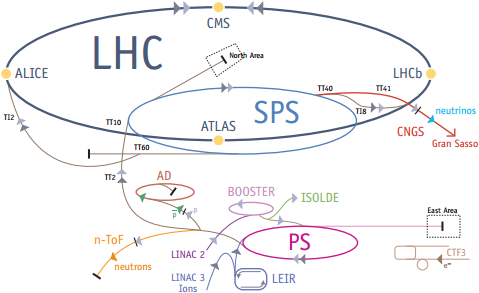
\includegraphics[width=300px]{lhcb/lhc.png}
\caption{\small The LHC Accelerator System}
\label{fig:lhc}
\end{figure}

The initial linear accelerator (LINAC2) accelerates protons energy to 50 MeV,
then they are fed through the Proton Synchrotron Booster (BOOSTER) which
accelerates them to 26 GeV, and finally protons are injected into the LHC
complex at an energy of 450 GeV.

The four main LHC experiments situated at the beam crossing points shown in
figure~\ref{fig:lhc}: \atlas, \alice, \cms, \lhcb. \alice dedicated to heavy
ion physics. \atlas and \cms are general purpose detectors, which primary goal is
to discover production of new particles. More details on the \lhcb experiment,
data from which is studied in this thesis, are given in the next section.

The new particles are expected to have large masses and their production
processes have small cross sections, so the LHC machine is designed with both
a center-of-mass energy and a luminosity as large as possible.

The operation of the \lhc can be shown as follows: two bunch of protons move in
opposite direction in orbit around 27\km circumference of the accelerator by
the magnetic field of superconducting magnets. A temperature 2\degk is preserved
for magnets' coils to generate a maximum magnetic field of 8\tesla. This field
allows to produce the design center-of-mass energy of $\sqs=14\tev$.
Finally the bunches are designed to collide with a frequency of 40\mhz at the
interaction points to archive a design luminosity of $10^{34}\cm^{-2}c^{-1}$.

The main LHC design parameters are shown in Table~\ref{tab:lhc}.

\begin{table}[t]
\caption{\small The main LHC design parameters}
\centering
\begin{tabular}{rr}
Circumference & 27\km\\
Center-of-mass energy & 14\tev\\
Injection energy & 450\gev\\
Field at 2 $\times$ 450\gev & 0.535\tesla\\
Field at 2 $\times$ 7\tev & 8\tesla\\
Helium temperature & 2\degk\\
Luminosity & $10^{34}\cm^{-2}s^{-1}$\\
Bunch spacing & 25\ns\\
Luminosity lifetime & 10\hr\\
Time between 2 fills & 7\hr\\
\end{tabular}
\label{tab:lhc}
\end{table}

\section{The LHCb}
\label{ch_lhcb:lhcb}

The \lhcb is an experiment dedicated to precision measurements of CP violation
and rare decays of hadrons containing beauty (b) and charmed (c) quarks as
an indirect search of new physics beyond the Standard Model.

The \lhcb detector is a forward single-arm spectrometer with forward angular
momentum coverage from 10 mrad to 300 mrad in the bending plane and 10 mrad to
250 mrad in the non-bending plane. The choice of the unique LHCb geometry is
justified by the fact, that b-hadrons are predominantly produced in narrow
angular cones in the same forward and backward directions.

\begin{figure}[tb]
\begin{center}
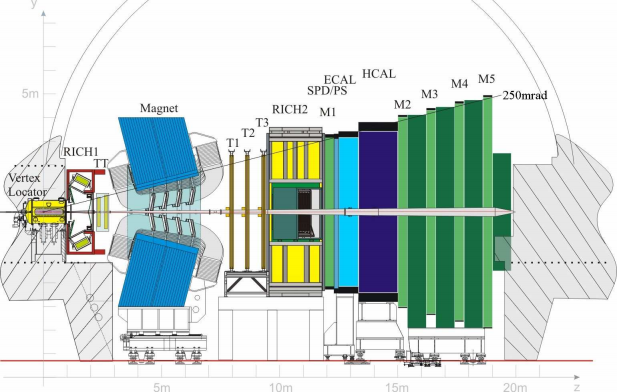
\includegraphics[width=300px]{lhcb/lhcb.png}
\end{center}
\caption{\small Schematic layout of the LHCb detector~\cite{Alves:2008zz}. 
The interaction point where the protons collide is on the left of the figure, 
and sub-detectors are labeled.}
\label{fig:lhcb}
\end{figure}

LHCb allows the full reconstruction of exclusive decays of the b- and c-hadrons
in a variety of leptonic, semi-leptonic and purely hadronic final states. 
In order to achieve this goal and extract the physics of interest, 
specialized sub-detectors involved within the LHCb detector to perform the 
following major tasks:

\begin{itemize}

\item {\bf Precision vertexing}: a sufficient separation between primary and 
secondary vertices is required to efficiently select b-hadron candidates 
and allow time dependent analyses to be performed. Such measurements are 
performed by the VErtex LOcator (\velo).

\item {\bf Invariant mass determination}: an finest invariant mass
resolution is required in order to maximize the significance of signal with
respect to background. Therefore, precision energy and momentum estimates of
reconstructed tracks must be performed. This is achieved by \lhcb’s tracking
and calorimetry systems.

\item {\bf Particle identification}: hadronic decays of b- and c-hadrons, 
having identical topology but different flavour content in the final state, 
may peak at a common invariant mass; additional information is required to 
distinguish them from one another. 
Discrimination between charged hadrons (particularly pions and kaons) is 
achieved with a high performance Ring Imaging CHerenkov (RICH) system, 
whilst electrons, photons and muons are identified via the 
Calorimeter and Muon systems, respectively.

\item {\bf Flexible and robust trigger and data acquisition}: this is required 
in order to cope with rapid changes in running conditions and physics 
interests. A dedicated multi-stage trigger, capable of selecting many different 
final states in an hadronic environment, reduces the data rate from the initial 
40\mhz of ``visible interactions'' to 5\khz which is suitable for 
offline storage and analysis.
\end{itemize}

Figure~\ref{fig:lhcb} presents the layout of the detector sub-systems 
within the LHCb detector. More details on each sub-detector will be given in 
the next sections.

\section{Tracking system}

The tracking system is an important part of the LHCb detector that collects such
information about charged particles as vertexing (determining the distance
between the production and the decay vertex of the $\chi_b$) and
momentum reconstruction. These two together used for reconstruction of the mass,
the angular and the proper time resolution, that are important for signal
selection and background suppression during the offline analysis of
$\chi_b \rightarrow \Upsilon \gamma$. Besides this, momentum and decay distance
information about momentum and decay distance are used in the trigger.

The LHCb tracking system is composed of a dipole magnet, the VELO and four 
planar tracking systems: the Tracker Turicensis (TT) upstream of the dipole 
magnet and three tracking stations T1, T2 and T3 downstream of the magnet. 
The latter three stations cover the entire geometrical acceptance of the 
spectrometer. To achieve the excellent tracking performance and also due to 
track multiplicity considerations, these three stations are composed of two 
distinct parts called the Inner Tracker (IT) and Outer Tracker (OT). 
The VELO, TT and IT use silicon strip technology while straw tubes are 
employed in the OT.\@ In fact, the TT and IT share a common technology, 
called collectively the Silicon Tracker (ST). They have a very similar layout
sharing the same silicon microstrip technology with a strip pitch
of $200\mum$. Each of the four ST stations is composed of four detector 
layers with the strip directions arranged in a so called x-u-v-x layout: 
the first and fourth layers have vertical readout strips, while second (u) 
and third (v) layers have the strips rotated by a stereo angle of $+5^\circ$ 
and $-5^\circ$ respectively. This layout is designed to have the best hit
resolution in the x direction (in the bending plane), without losing the 
stereo measurement of the tracks.

\subsection{Vertex Locater}

To provide precise measurements of track coordinates close to the interaction 
region, the Vertex Locator (VELO), consisting of a series of silicon modules, 
is arranged along the beam direction. It is used to identify the detached 
secondary vertices typical for b-hadron decays and makes it possible to meet 
the requirement to reconstruct $\chi_b \rightarrow \Upsilon \gamma$ decays
with a proper time resolution good enough to resolve the fast time-dependent
oscillations of the CP asymmetry.

To provide accurate measurements of the position of the vertices, the silicon
modules of the VELO are placed closed to the beam axis, namely at 8\mm.
In order to detect the majority of the tracks originating
from the beam spot ($\sigma$ = 5.3\cm), the detector is designed such that
tracks emerging up to $z = 10.6\cm$ downstream from the nominal interaction
point cross at least 3 VELO stations, for a polar angular window between 15
and 300\mrad, as shown in Figure~\ref{fig:velooverview}.

\begin{figure}[tb]
\begin{center}
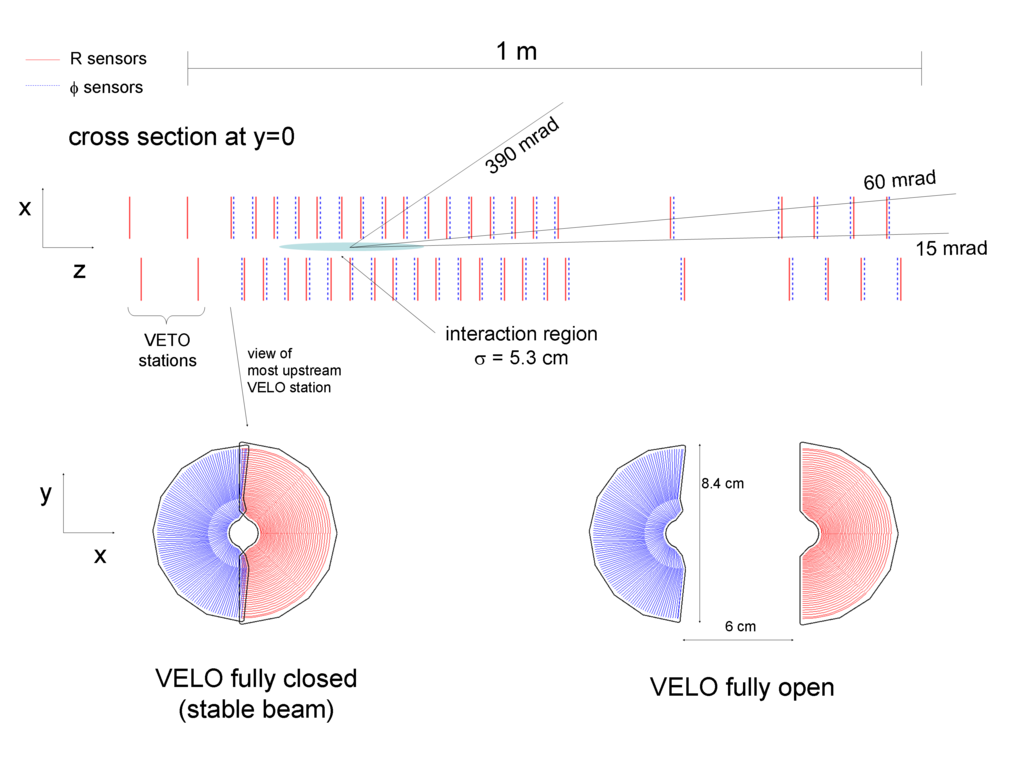
\includegraphics[width=300px]{lhcb/velooverview.png}
\end{center}
\caption{\small The setup of the VELO silicon modules along the beam direction.
The left two pairs form the pile-up system. Indicated are the average crossing
angle for minimum bias events (60\mrad), and the minimal (15\mrad) and
maximal (390\mrad) angle for which at least 3 VELO stations are crossed.
390\mrad is the opening angle of a circle that encloses a rectangular opening
angle of 250 $\times$ 300\mrad}
\label{fig:velooverview}
\end{figure}

To enable fast reconstruction of tracks and vertices in the \lhcb trigger,
a cylindrical geometry with silicon strips measuring $r\phi$ coordinates is
chosen for the modules.

The strips of the r sensor are concentric semi-circles, the $\phi$ sensors 
measure a coordinate almost orthogonal to the r-sensor. The geometry is shown in
Figure~\ref{fig:velomodule}. A 2D reconstruction in the r-z plane alone allows to
detect tracks originating from close to the beam line in the high-level trigger.
These measurements are used to compute the impact parameter of tracks with
respect to the production vertex, which is used in the trigger to discriminate 
between signal and background. The level-0 trigger uses information from the
pile-up veto system, two stations located upstream, which make it possible to
reject events with multiple pp interactions in one beam crossing.

\begin{figure}[H]
  \setlength{\unitlength}{1mm}
  \centering
  \resizebox{\textwidth}{!}{
  \begin{picture}(150,80)
    \put(0,0){
        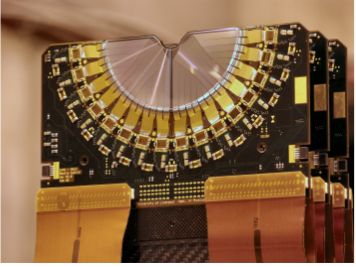
\includegraphics[width=.45\textwidth]{lhcb/velosensor}
    }
    \put(75,0){
        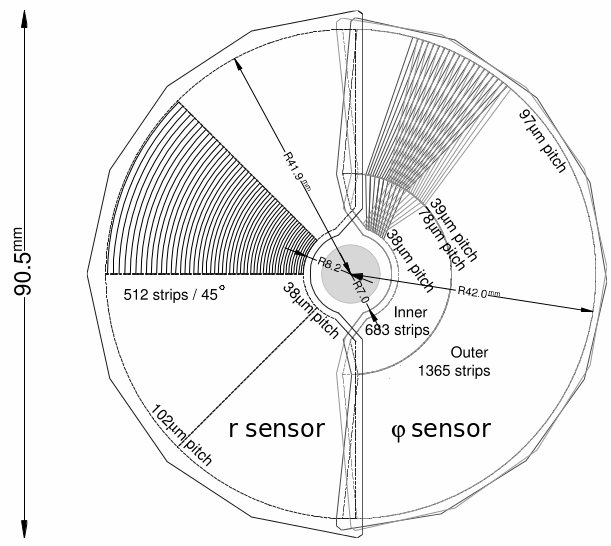
\includegraphics[width=.45\textwidth]{lhcb/velomodule}
    }
  \end{picture}
  }
\caption{The \velo r-sensors (left) and $\phi$-sensors (right).}
\label{fig:velomodule}
\end{figure}




The setup of the \velo is as follows. The half disc sensors are arranged in
pairs of r and $\phi$ sensors and are mounted back-to-back. The sensors are 300
$\mu m$ thick, radiation tolerant, n-implants in n-bulk technology. The
minimal pitch of both the r and the $\phi$ sensors is 32 $\mum$, linearly
increasing towards the outer radius at 41.9 mm. To reduce the strip occupancy
and pitch at the outer edge of the $\phi$-sensors, the $\phi$-sensor is divided
in two parts. The outer region starts at a radius of 17.25 mm and has
approximately twice the number of strips as the inner region. The strips in
both regions make a $5^\circ$ stereo angle with respect to the radial to
improve pattern recognition, and adjacent stations are placed with opposite
angles with respect to the radial. In order to fully cover the azimuthal angle
with respect to the beam axis, the two detector halves overlap, as is shown in
Figure~\ref{fig:velomodule}.

For reason to minimize the amount of material between the particle vertices
active detector layers the detector is placed inside vacuum. To separate the
primary beam vacuum from the secondary vessel vacuum and shield the detector
from RF pickup from the beam, the sensors are separated from the beam vacuum by
a thin aluminium foil. Both the sensors and this commonly named RF-foil are
contained inside a vacuum vessel. During beam injection the two halves of the
VELO are retracted 3\cm away from the nominal beam position. The RF-foil is
designed to minimize interactions.

\subsection{Magnet}

To provide a good momentum resolution, the \lhcb experiment utilizes a (dipole)
magnet (see Figure~\ref{fig:magnet}), which bends the tracks of charged
particles. The not superconducting magnet consists of two saddle-shaped coils.
These are placed mirror symmetrically, such that the gap left open by the
magnet is slightly larger than the \lhcb acceptance, and the principal field
component is vertical throughout the detector acceptance.

\begin{figure}[tb]
\begin{center}
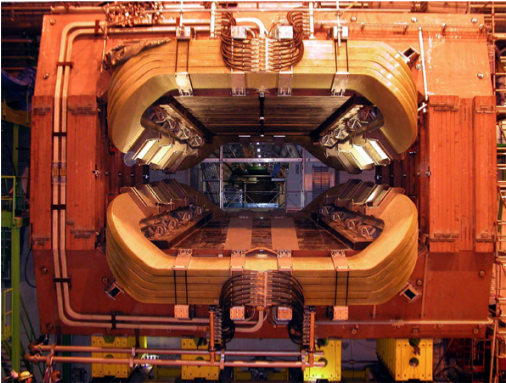
\includegraphics[width=300px]{lhcb/magnet}
\end{center}
\caption{\small The \lhcb dipole magnet. The proton-proton interaction
region lies behind the magnet.}
\label{fig:magnet}
\end{figure}


The quantity important for momentum resolutions, and hence for the analysis of
$\chi_b \rightarrow \Upsilon \gamma$ channel, is the integrated magnetic field
the magnet delivers. For tracks passing through the entire tracking system this
is
\cite{Alves:2008zz}:   

$$ \int Bdl = 4 Tm $$ making it possible to measure charged particles’ momenta
up to 200\gev within 0.5\% uncertainty.

\subsection{Inner tracker}

\begin{figure}[tb]
\begin{center}
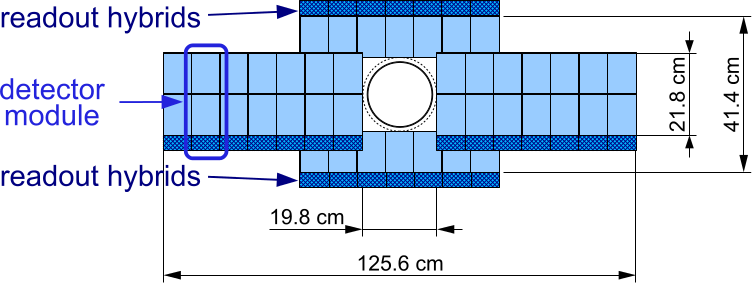
\includegraphics[width=300px]{lhcb/veloit}
\end{center}
\caption{\small Layout of the \intr.}
\label{fig:veloit}
\end{figure}

To perform accurate momentum estimates, important for mass, angular and proper
time resolutions in the reconstruction of the $\chi_b \rightarrow \Upsilon
\gamma$ channel, hit information downstream of the magnet is required, which is
provided by three tracking stations. Since the magnet bends particles in the
horizontal direction perpendicular to the beam pipe, the track density is
largest in an elliptically shaped region around the beam pipe. In order to have
similar occupancies over the plane, a detector with finer detector granularity
is required in this region. Therefore, the Inner Tracker (IT), 120\cm wide and
40 cm high, as shown in Figure~\ref{fig:veloit}, is located in the center of
the three tracking stations.



Due to the high track density near the beam pipe, silicon strip detectors are
used. The total active detector area covers 4.0 $m^2$, consisting of 129024
readout strips of either 11\cm or 22\cm in length. To improve track
reconstruction, the four detector layers are arranged in an x-u-v-x geometry,
in which the strips are vertical in the first and in the last layer, whereas
the other two (u, v) layers are rotated by stereo angles of $\pm5^\circ$,
providing the sensitivity in the vertical direction.

The pitch of the single-sided $p^+$-on-n strips is $198\mum$. In order to have
similar performance in terms of signal-to-noise, the thickness of the sensors
is $320\mum$ for the single-sensor ladders below and above the beam pipe, and
$410\mum$ for the double sensors at the sides of the beam pipe. The four
layers are housed in 4 boxes, which are placed such that they overlap. These
overlaps avoid gaps in the detector and, more importantly, make it possible to
perform alignment using reconstructed tracks.



\subsection{Outer tracker}

Similar to the \intr, the Outer Tracker (\ot) performs track measurements
downstream of the magnet, allowing to determine the momenta of charged
particles. The OT covers the outer region of the three tracking stations T1--T3.

Since the track density further away from the beam pipe is lower, straw tubes
are used. The total active area of one station is $5971\times4850\mm^2$, and
the \ot and the \intr together cover the full acceptance of the experiment. As is
the case for the \intr, these layers are also arranged in an x-u-v-x geometry, as
shown in Figure~\ref{fig:veloot}.

\begin{figure}[tb]
\begin{center}
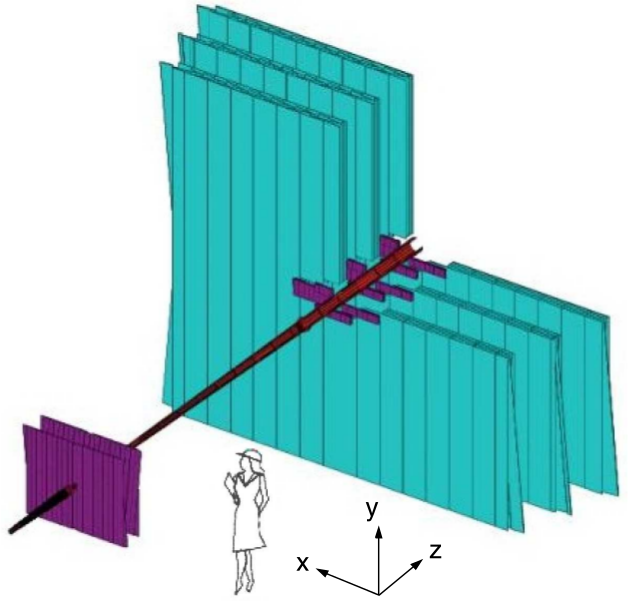
\includegraphics[width=300px]{lhcb/veloot}
\end{center}
\caption{\small Layout of the OT.}
\label{fig:veloot}
\end{figure}

The OT is designed as an array of individual, gas-tight straw-tube modules.
Each module contains two layers of drift-tubes with an inner diameter of
4.9\mm. The front-end (FE) electronics measures the drift time of the
ionization clusters produced by charged particles traversing the straw tubes,
digitizing it with respect to every bunch crossing. Given the bunch crossing
rate of 25\ns and the diameter of the tube, and in order to guarantee a fast
drift time (below 50\ns) and a sufficient drift-coordinate resolution
(200\mum), a mixture of Argon (70\%) and CO2 (30\%) is used as counting gas.

\subsection{Tracker Turicensis}

To improve the momentum estimate of charged particles, track measurements are
performed before these enter the magnet. Therefore, the Tracker Turicensis
(TT), a planar tracking station, is located between the VELO and the LHCb
dipole magnet. It is also used to perform the track measurements of long lived
neutral particles which decay after the VELO.\@ In addition, by using the weak
magnetic field inside the tracker, track information from the TT is used by the
High Level Trigger to confirm candidates between the VELO and the tracking
stations.

In order to cover the full acceptance of the experiment, the TT is constructed
150 cm wide and 130 cm high. It consists of four detector layers, with a total
active area of $8.4\m^2$, with 143360 readout channels, up to 38\cm in length.
To improve track reconstruction, the four detector layers are arranged in two
pairs that are separated by approximately 27\cm along the \lhcb beam axis. And
again, like the IT and the OT, the TT detection layers are in an x-u-v-x
arrangement.

\begin{figure}[tb]
\begin{center}
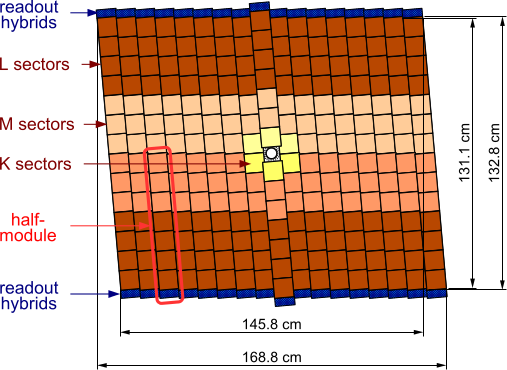
\includegraphics[width=300px]{lhcb/velott}
\end{center}
\caption{\small Layout of one of the stereo plane detector layers of the \ttracker}
\label{fig:velott}
\end{figure}


The layout of one of the detector layers is illustrated in
Figure~\ref{fig:velott}. Its basic building block is a half module that covers
half the height of the \lhcb acceptance. It consists of a row of seven silicon
sensors, named a ladder. The silicon sensors for the \ttracker are $500\mum$
thick, single sided $p^+$-on-n sensors, as for the IT.\@ They are
$9.64\cm\times9.44\cm$ long and carry 512 readout strips with a strip pitch of
$183\mum$.

\section{Particle identification}

Particle identification (PID) is a fundamental requirement for \lhcb. It is
essential for the goals of the experiment to separate pions from kaons in
selected B hadron decays.

\subsection{\rich system}

There are two \rich detectors in \lhcb. \richone is located before the magnet
(between the \velo and \ttracker) and are used for identification of low momentum
particles. RICH2 is located behind the magnet (between \ot and M1) and is
used for the identification of high momentum particles. The combination of both
detectors allows for kaon and pion separation in the momentum range $2 < p <
100 \gevc$.

\begin{figure}[tb]
\centering
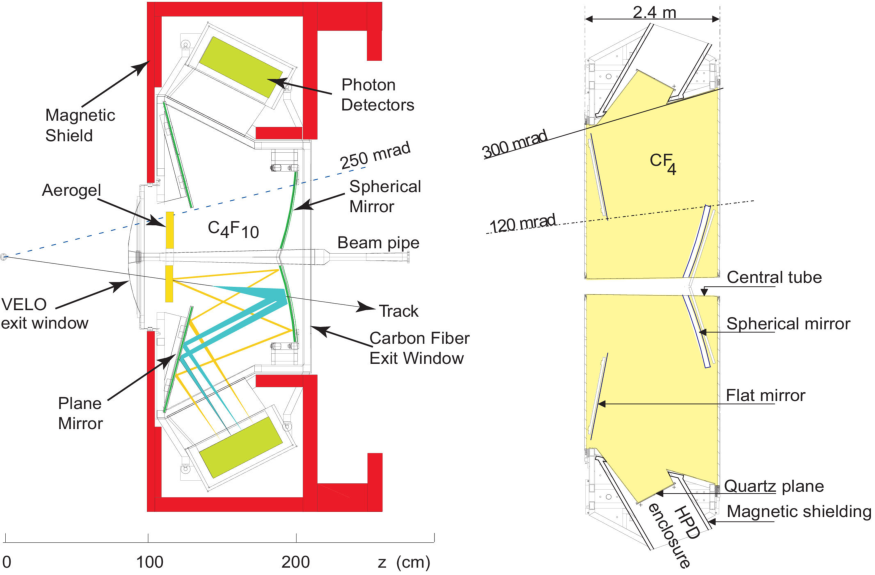
\includegraphics[width=.75\textwidth]{lhcb/rich}
\caption{\small Layout of the \richone(left) and \richtwo(right) detectors.}
\label{fig:rich}
\end{figure}

The RICH detectors measure the opening angle of the Cherenkov emission cone
produced by a charged particle that traverses the medium. The photon emission
is focused on the detector surface using a combination of spherical and flat
mirrors. The mirrors are tilted to allow the photo detectors to be positioned
outside the active area of the detector.

The Cherenkov emission angle $\theta$ is given by:
$$\cos\thetaθ = \frac{1}{n\beta}$$
\noindent where n is the refractive index of the radiator medium and 
$\beta = v/c$ is the velocity of the particle. Given the momentum p of a
particle and the emission angle $\theta$, the particle mass and therefore the
type can be determined.

The \richone and \richtwo detectors have different effective momentum ranges,
which are determined by the corresponding radiator emission threshold velocity
$\beta_{thr} = 1/n$. The \richone detector uses a combination of aerogel and
$C_4F_{10}$ gas radiators and covers the low momentum range $1<p<60 \gevc$. The
\richtwo detector uses a $CF_4$ radiator and covers the high momentum range $15
< p < 100 \gevc$.

\subsection{Muon system}

The \lhcb muon system is designed for muon identification and tracking. It
provides information on the transverse energy of the muon to the first level
trigger (L0) and muon-ID for the second level trigger (HLT) and offline
analysis.

\begin{figure}[tb]
\begin{center}
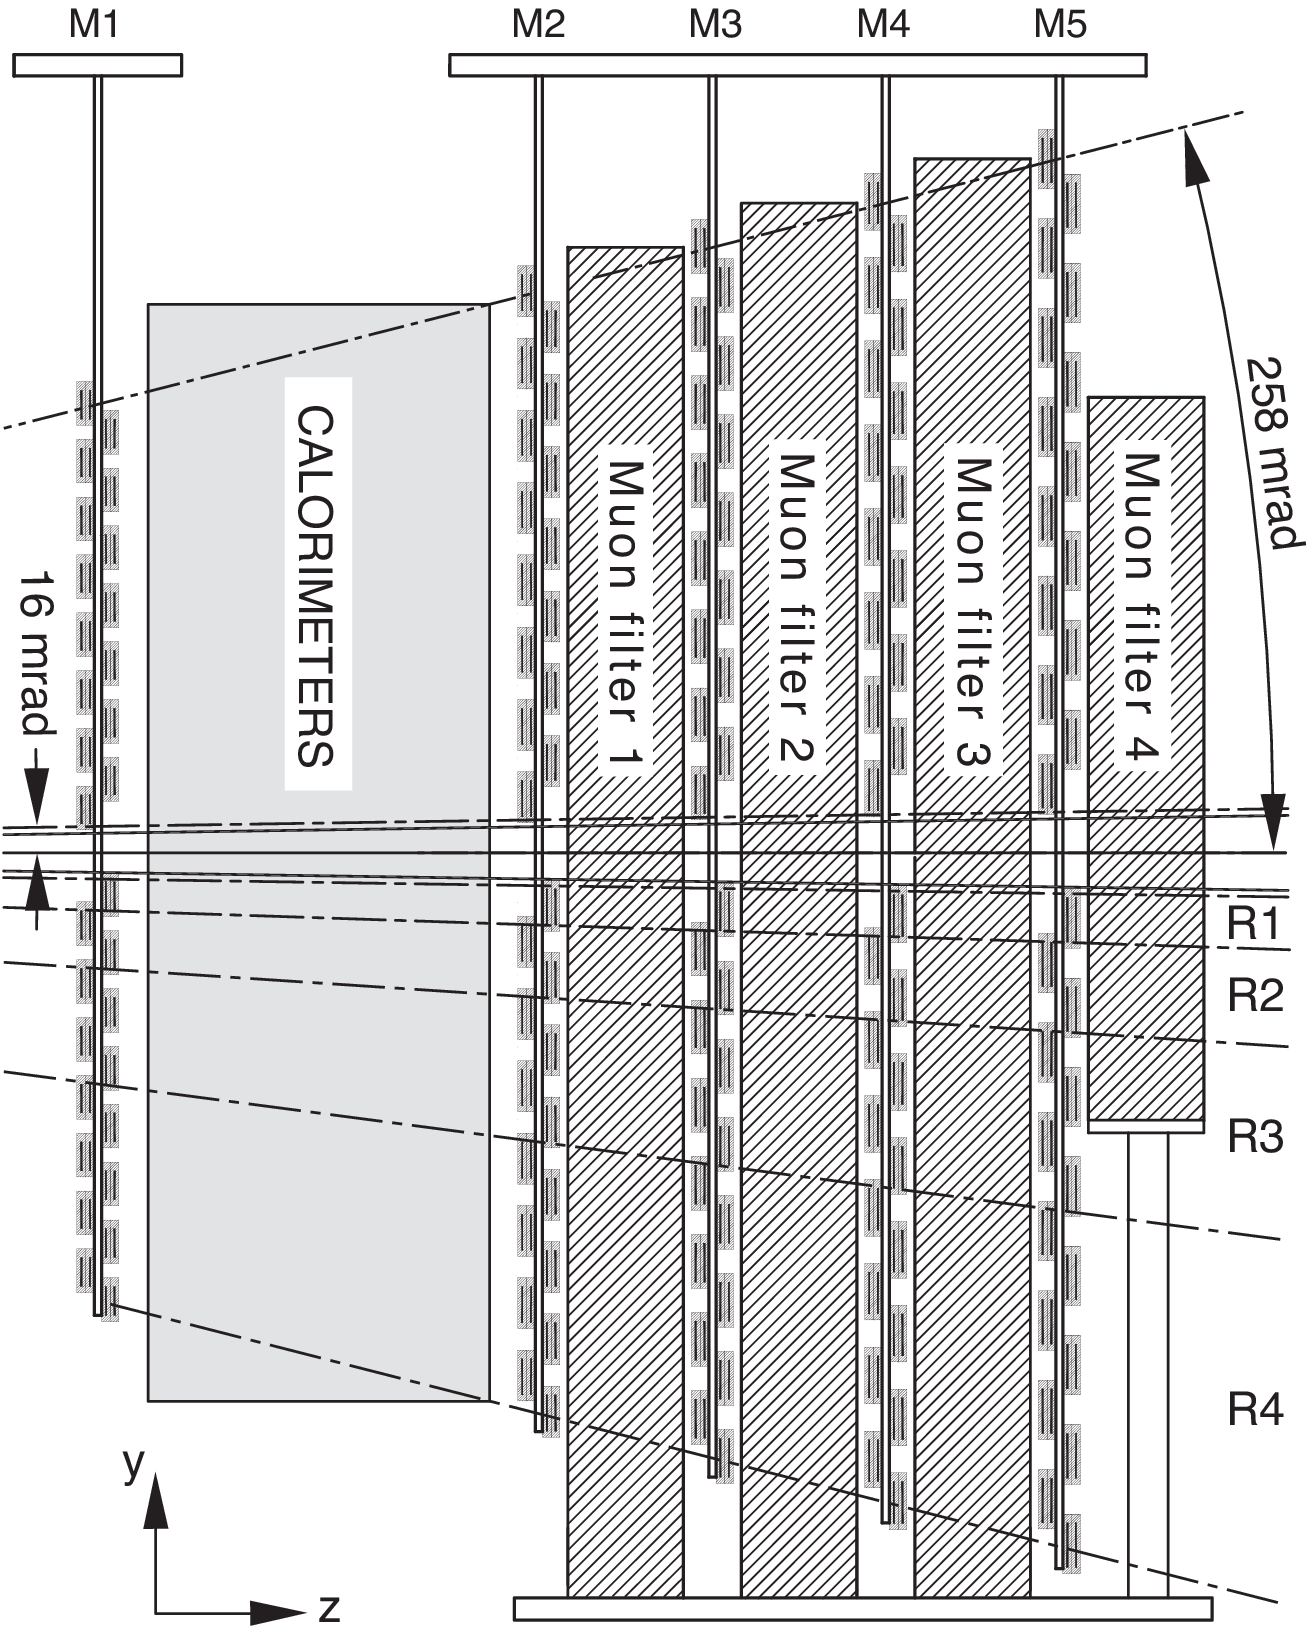
\includegraphics[width=.75\textwidth]{lhcb/muon}
\end{center}
\caption{\small Layout of the muon system.}
\label{fig:muon}
\end{figure}

The muon system is composed of five stations (M1--M5) placed along the
beam axis (Figure~\ref{fig:muon}). Stations M2 to M5 are placed downstream of the
calorimeters and are interleaved with iron absorbers. The M1 station is
located in front of the \spd/\presh and is used to improve the transverse momentum
estimate in the trigger. Each station is divided into four regions, R1 to R4,
with increasing distance from the beam axis. The granularity of each region is
made according to the particle flux, keeping the channel occupancy roughly
constant over the four detector regions. For more precise momentum measurement
the granularity is higher in the horizontal plane.

\subsection{Calorimeter system}

The calorimeter system is designed to measure the energy and position of
hadrons, electrons and photons. This information is used in the first level
trigger (L0) as well as in the offline analysis.

The calorimeter system is located between the RICH2 and muon detectors and
consists of a scintillator pad detector (SPD), a pre-shower detector (\presh), an
electromagnetic calorimeter (\ecal) and a hadronic calorimeter (\hcal). The \spd
and PS are located in front of the \ecal and provide information on the
evolution of the electromagnetic shower. The \ecal serves to measure the energy
of electrons and photons, whereas the \hcal measures the energy of hadrons.

When a particle hits the calorimeter, it produces a cascade of secondary
particles. These secondary particles excite the scintillator material, which in
turn emits the scintillation light. The light is transmitted through
wavelength-shifting fibers to the photomultiplier tubes. The total amount of
light collected by photomultipliers is proportional to the energy of the
incident particle.

The SPD and PS consist of scintillator pads, separated by a 15\mm thick lead
converter. The SPD is used for identification of charged particles before the
start of the shower. The lead converter initiates the shower that subsequently
is detected by the PS.\@ The SPD allows to separate electrons from photons,
whereas the PS is used for separation of electrons and photons from hadrons.

The ECAL consists of lead-scintillator modules and covers the acceptance of
$25<\theta_x< 300\mrad$ and $25 < \theta_y < 250\mrad$ in the horizontal and
vertical planes, respectively. Each module is 42\mm thick and consists of
alternating layers of 4\mm scintillator material and 2\mm lead absorber. The
modules vary in size from $4\times4\cm^2$ in the inner part of the detector, to
$6\times6\cm^2$ in the middle and $12\times12\cm^2$ in the outer part of the
detector. The energy resolution of \ecal for electrons and photons is: 

\begin{equation}
\left(\frac{\sigma_{E}}{E}\right)_{\ecal} = \frac{10\%}{\sqrt{E\left[\gev\right]}} \oplus 1\%
\label{eqn:ecal}
\end{equation}

The HCAL is located behind the \ecal. The modules of the HCAL have dimensions of
$13\times13\cm^2$ and $26\times26\cm^2$ in the inner and outer part of the
detector, respectively, and consist of alternating layers of 1\cm thick iron
and scintillators. The energy resolution of \hcal for hadrons is:

\begin{equation}
\left(\frac{\sigma_{E}}{E}\right)_{\hcal} = \frac{80\%}{\sqrt{E\left[\gev\right]}} \oplus 10\%
\label{eqn:ecal}
\end{equation}

\section{Trigger}

The \lhcb trigger system is used for the selection and storage of events for
LHCb physics studies. The general layout of the trigger is shown in Fig. 2.12.
The first level trigger Level-0 (L0) is implemented in hardware. The L0 trigger
decision is based on the information of the calorimeter and muon systems. Both
systems provide information on the multiplicity, and transverse energy \et or
transverse momentum \pt of individual particles. The High Level Trigger (HLT)
is the second level trigger of \lhcb. The HLT is a software trigger that runs on
about 15000 processors of the Event Filter Farm. The HLT, with its two stages
HLT1 and HLT2, reduces the 1\mhz L0 rate to about 5\khz which is put on
storage.

HLT1 reduces the rate from 1\mhz to 50\khz. HLT1 performs the reconstruction
of particles in the \velo and determines the location of primary vertexes and
impact parameters (IP) of the particles. The events are selected based on the
presence of particles which pass the requirements on the minimum track quality,
IP, momentum, and transverse momentum. These selections are based on the decay
kinematics of charm and beauty hadrons, such as:

\begin{itemize}
\item high average momentum and transverse momentum of charm and beauty
hadrons, and consequently their decay products;
\item the decay vertex is well displaced from the collision (primary) vertex, and
consequently the reconstructed final state particles on average do not point
to the primary vertex.
\end{itemize}

HLT2 reduces the rate from 50\khz to 3\khz and is mainly based on inclusive
trigger lines that cover most of the B decays with displaced vertexes. In
addition, HLT2 contains trigger lines based on the presence of muons and lines
aiming at selecting exclusive B decays. HLT2 uses similar requirements on the
particles as HLT1, in addition to which the requirements on distance between
primary and secondary vertexes, vertex quality, mass and lifetime are used.

\section{LHCb 2010--2012 operation}

In 2010 and 2011, \lhcb operated at center-of-mass energy \sqs=7\tev. In 2012
--- at \sqs=8\tev. Figure~\ref{fig:lumi} shows the integrated luminosity
delivered and recorded by LHCb in these data-taking periods. In 2011 and 2012,
the operation conditions and luminosity were relatively stable and the total
recorded luminosity amounts to 1.107\invfb and 2.082\invfb in 2011 and 2012
correspondingly.

The data used in the analysis of $\chi_b$ production presented in this thesis
correspond to the full datasets collected in 2011 and 2012 years.

\begin{figure}[tb]
\begin{center}
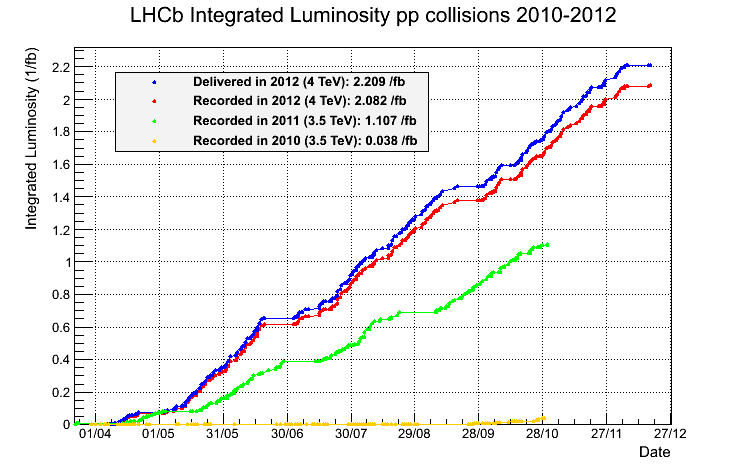
\includegraphics[width=.75\textwidth]{lhcb/lumi}
\end{center}
\caption{\small \lhcb integrated luminosity pp collisions 2010--2012.}
\label{fig:lumi}
\end{figure}